\section{Opportunities for advanced control}

\subsection{Model Predictive Control}
Model Predictive control is an advanced control technique that can cope with complex multivariate control problems. A model predictive controller (MPC) functions by taking in current measurements of manipulated variables (MVs) and disturbances (DVs) from the plant and then calculates the future profile for the controlled variables (CVs) and constraint variables in order to predict the optimal values for the manipulated variables. The controller performs two sets of calculations, first to determine the future profile of CVs ('set-point calculations'), and second the optimal values for MVs ('control calculations') to reach the desired set-points. 

The future profile of CVs are calculated from solving an optimisation problem that determines the set points for the CVs for a period of time in the future ('prediction horizon'). The objective function for this optimisation is usually to maximise profit or minimise cost, and is subject to inequality constraints that can vary with time such as variations in process conditions, functional instrumentation and economic data such as pricing. These set-points are re-calculated each time new data is received. The optimal values for MVs are then calculated. Unlike traditional PID controllers, a sequence of MV steps are calculated by splitting the prediction horizon into a number of sampling intervals, and the effects on CVs are determined in order to move them closer to the desired set-points (see Figure \ref{MPC}). 

    \begin{wrapfigure}{r}{0.6\linewidth}
        \centering
        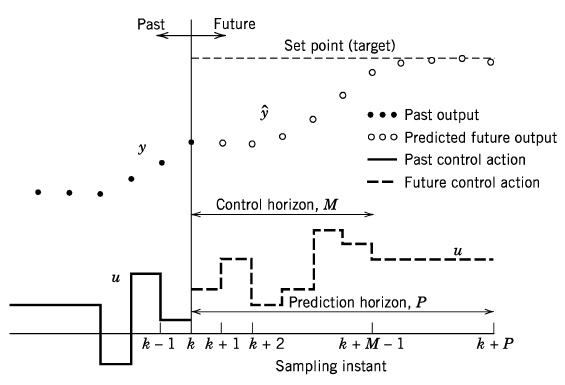
\includegraphics[width=\linewidth]{chapters/4-operation-control/4-Figures/MPC-Seborg-2011.png}
        \caption{Illustration of MPC in action, taken from \textcite{}. $u$ is a manipulated variable, and $y$ is a controlled variable}
        \label{fig:MPC}
    \end{wrapfigure}

The goal of the MPC is to minimise the differences between the set-point and the predicted values of the CV at each sampling instant. Expressing these errors in a vector to the MPC algorithm returns a combination of MV steps with minimised total error. 


\subsection{Real-time control}